	\documentclass[10pt]{scrartcl}

\usepackage[utf8]{inputenc}
\usepackage{tabularx}
\usepackage[ngerman]{babel}
\usepackage[automark]{scrpage2}
\usepackage{amsmath,amssymb,amstext}
%\usepackage{mathtools}
\usepackage[]{color}
\usepackage[]{enumerate}
\usepackage{graphicx}
\usepackage{lastpage}
\usepackage[perpage,para,symbol*]{footmisc}
\usepackage{listings} 
\usepackage[pdfborder={0 0 0},colorlinks=false]{hyperref}
\usepackage[numbers,square]{natbib}

\lstset{numbers=left, numberstyle=\tiny, numbersep=5pt, breaklines=true, showstringspaces=false} 

%changehere
\def\titletext{Praktikum 1 : Modellierung von Raumgestalten}
\def\titletextshort{Praktikum 1}
\author{André Harms, Oliver Steenbuck, Armin Steudte, Carsten Nötzel, Dennis Blauhut, Torben Becker}

\title{\titletext}

%changehere Datum der Übung
\date{26.10.2011}

\pagestyle{scrheadings}
%changehere
\ihead{MI, Thiel Clemen}
\ifoot{Generiert am:\\ \today}

\cfoot{Oliver Steenbuck \\ Andre Harms \\  Armin Steudte \\ Carsten Nötzel \\ Dennis Blauhut \\ Torben Becker}

\ohead[]{\titletextshort}
\ofoot[]{{\thepage} / \pageref{LastPage}}

\setlength{\parindent}{0.0in}
\setlength{\parskip}{0.1in}

\begin{document}
\maketitle

\setcounter{tocdepth}{3}
\tableofcontents
\listoffigures
\lstlistoflistings

\section{Einleitung}

\section{Räumliche Darstellung}

      \begin{figure}[htbp]
        \centering
                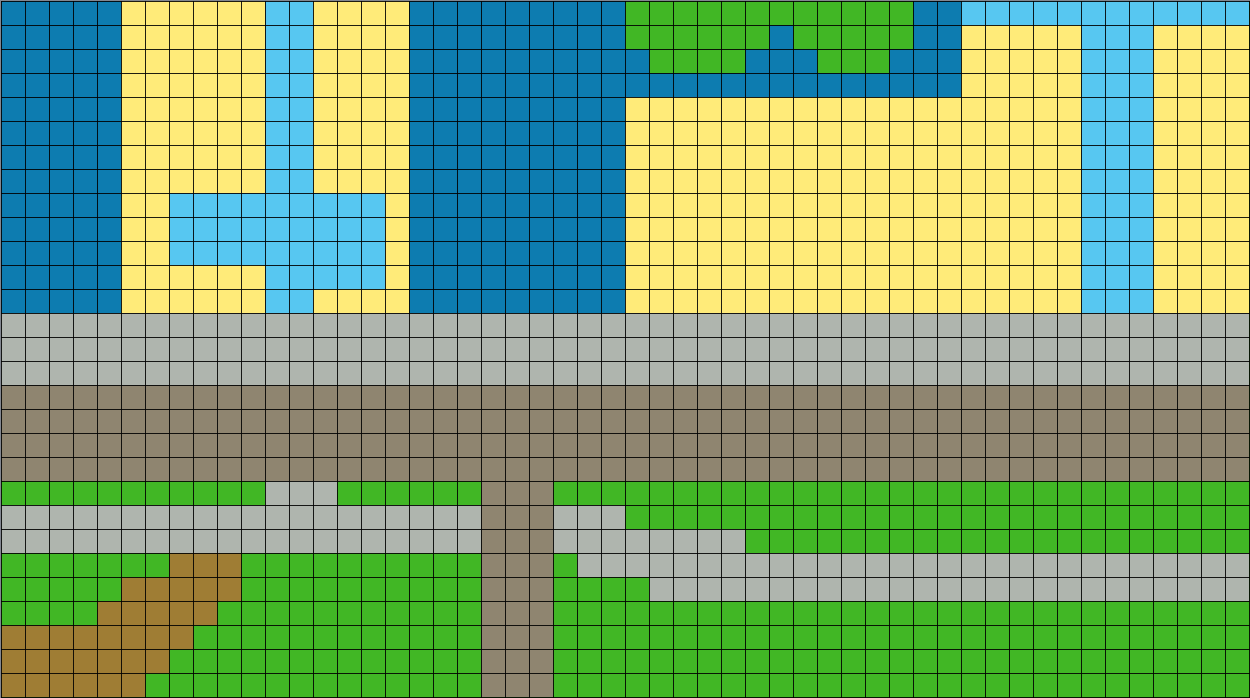
\includegraphics[scale=0.5]{img/tile_map_campus_pic}
        \caption{Ausschnitt von Campus als \glqq Tilebased Map\grqq{}}
        \label{img:tile_map}
        \end{figure}  
        
      
        
      \begin{figure}[htbp]
        \centering
                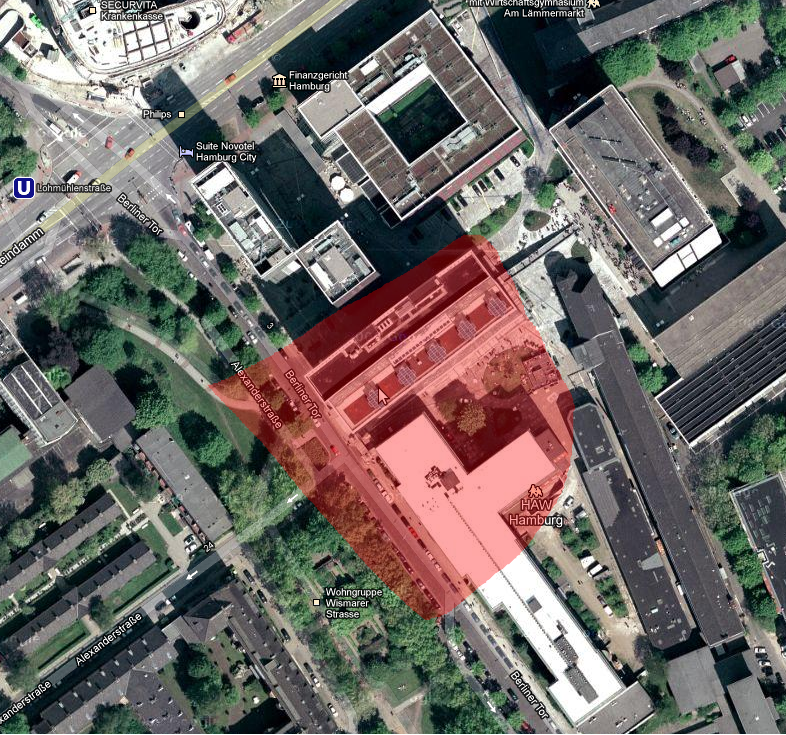
\includegraphics[scale=0.5]{img/google_maps}
        \caption{Ausschnitt Google-Maps}
        \label{img:google_maps}
        \end{figure}  

\section{Entitäten}

\section{Ebenen}



\end{document}

